%************************************************
\chapter{Results}\label{p03:results}
%************************************************
In this section, a series of iterative experiments were performed to find the best implementation/settings of the algorithm. As explained in chapter \ref{p02:session_tracking}, a wrong value of the "session\_timeout" parameter can produce different and perhaps incorrect results.

\section{Reading session experiments}
The reading session tracking is the most complex to model, because there are multiple internal and external variables to consider. First, we must define what actions are relevant to detect, in order to consider them as part of the learning process, and which ones are not (\Ie the user trying to game the system). Second, with the events already defined, we must determine how much time can pass between them, which is still part of the same reading/learning session.

\subsection{Baseline}
For the first iteration, the initial set of \textbf{opening, interaction and closing events} were defined as listed in table \ref{tb:event_type_v1}.

\begin{table}[htb]
	 \begin{tabularx}
	{\textwidth}{Xll}\toprule
		  \tableheadline{Event} & \tableheadline{Action type} \\ 
		\midrule 
		UMR - ARTICLE CLOSED & Closing \\ 
		\hline 
		UMR - CHANGE ORIENTATION & Interaction \\ 
		\hline 
		UMR - CLOSE ALTERMENU & Interaction \\ 
		\hline 
		UMR - OPEN ALTERMENU & Interaction \\ 
		\hline 
		UMR - SEND SUGGESTION & Interaction \\ 
		\hline 
		UMR - SPEAK TEXT & Interaction \\ 
		\hline 
		UMR - TRANSLATE TEXT & Interaction \\ 
		\hline 
		UMR - UNDO TEXT TRANSLATION & Interaction \\ 
		\hline 
		UMR - ARTICLE FOCUSED & Opening \\ 
		\hline 
		UMR - OPEN ARTICLE & Opening \\ 
		\hline 
		UMR - OPEN STARRED ARTICLE & Opening \\ 
		\hline 
		UMR - ARTICLES REQUESTED FROM ZEEGUU & Closing \\ 
		\hline 
	\end{tabularx} 
	\caption{User events classification, first iteration}\label{tb:event_type_v1}
\end{table}

For the \textbf{session\_timeout}, the initial test was done with 5 minutes.

By observing the total reading time by user, we can see that the highest value is 2120 minutes (roughly 1.4 days) and an average time of 11 minutes spent by the user with the longest average reading time. Additionally, by analyzing the daily activity for a specific user, we find long reading sessions spanning up to 1:20 hours long. Figure \ref{fig:visualizations_1st_iteration} show these results.

\begin{figure}[bth]
	\myfloatalign
	\subfloat[Total read time by user]
	{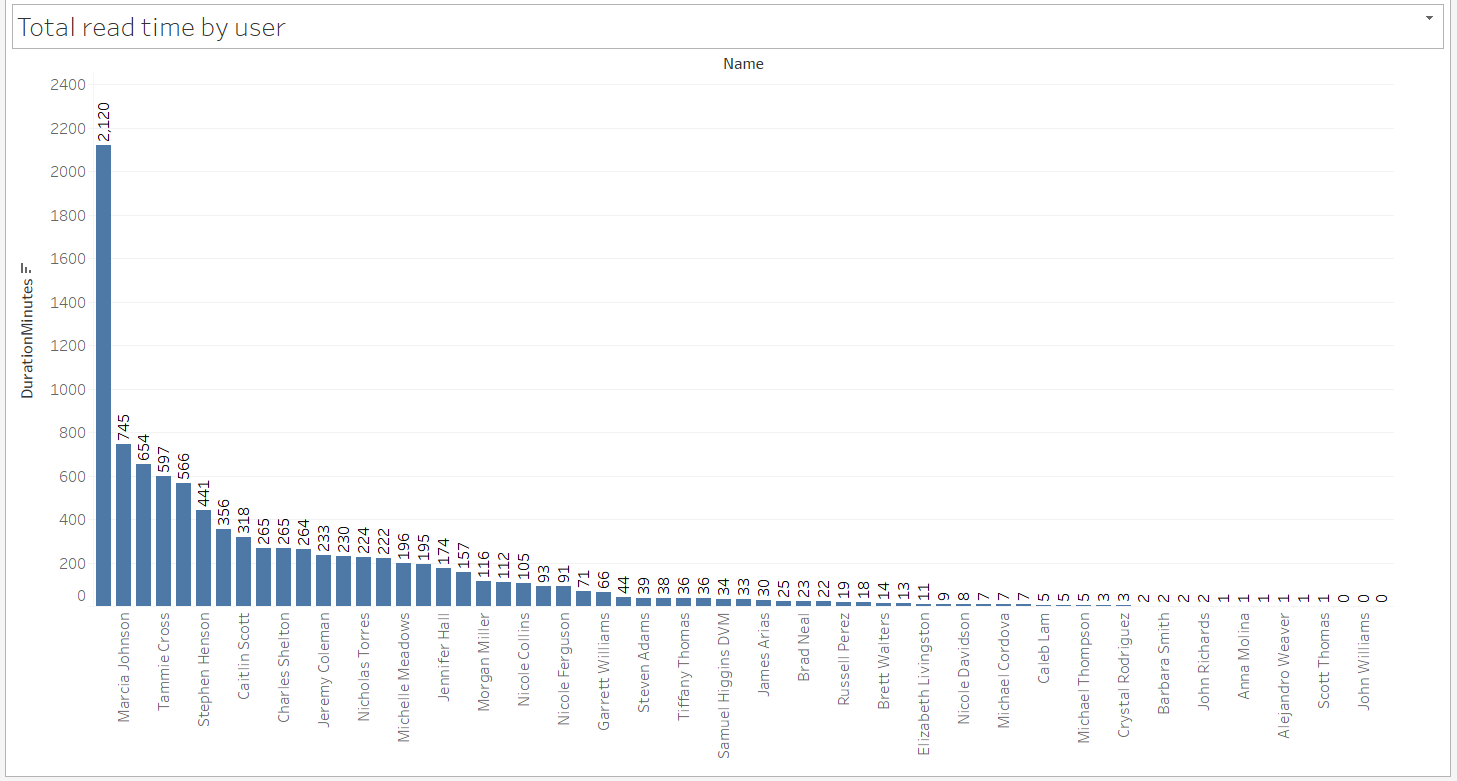
\includegraphics[width=.45\linewidth]{gfx/total_read_time_5_min_no_scroll}\label{fig:total_read_time_5min_no_scroll}} \quad 
	\subfloat[Average read time by user]
	{
		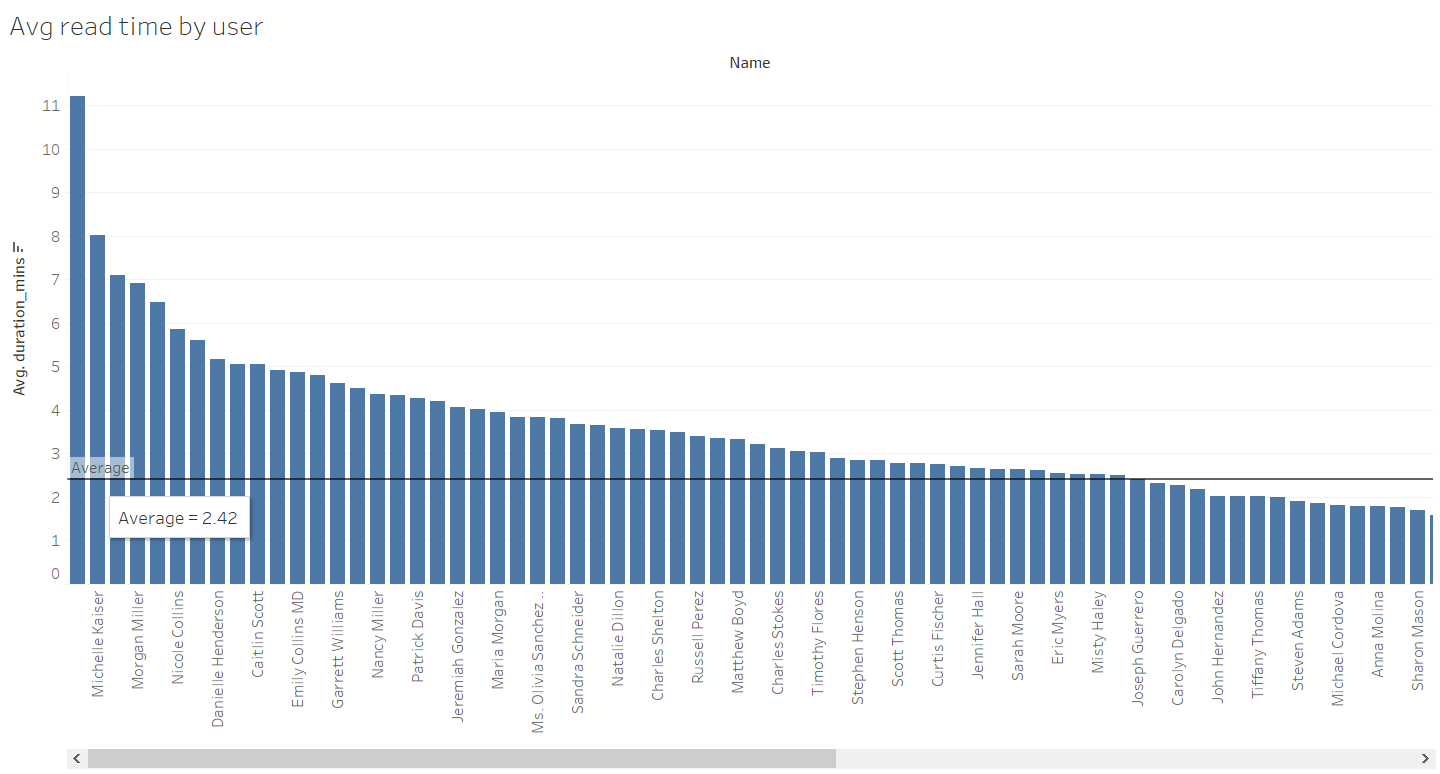
\includegraphics[width=.45\linewidth]{gfx/avg_read_time_5_min_no_scroll}\label{fig:avg_read_time_5_min_no_scroll}} \\
	\subfloat[Daily activity timeline]
	{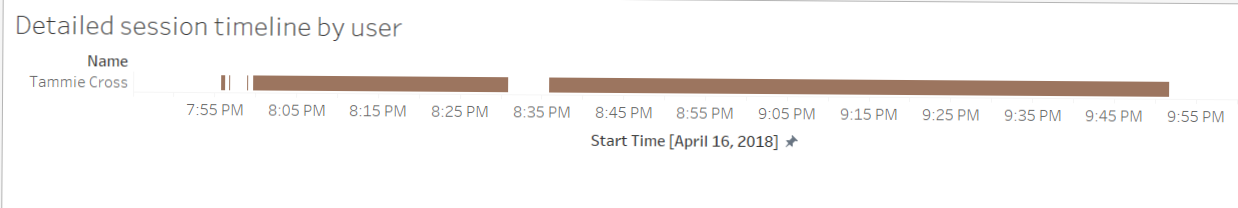
\includegraphics[width=.75\linewidth]{gfx/detailed_session_timeline_by_user_5min_no_scroll}\label{fig:detailed_session_timeline_by_user_5min_no_scroll}} \quad
	\caption{Reading session visualizations for session\_timeout of 5 minutes.}\label{fig:visualizations_1st_iteration}
\end{figure}


\subsection{Improving the baseline}
Using the previous settings as a baseline, the next idea was to reduce the value of session\_timeout, because the additional time benefit of 5 minutes might be too much of a consideration for a user reading without doing any action. For that to be possible, \textbf{scrolling events} were included as interaction events, so that they keep the session alive. Scrolling events are helpful for detecting more user activity, but they can be overwhelming for the web server and the database, for that reason, the event posting was limited to maximum 1 per second.

One of the interesting findings in the first iteration is the mean of the average read time for all the users(figure \ref{fig:avg_read_time_5_min_no_scroll}), we can observe that the average reader works for about 2.42 minutes. Taking this discovery into consideration plus scroll detection, we reduced the value of \textbf{session\_timeout} to 2 minutes and ran a second iteration of experiments.


\begin{figure}[bth]
	\myfloatalign
	\subfloat[Total read time by user]
	{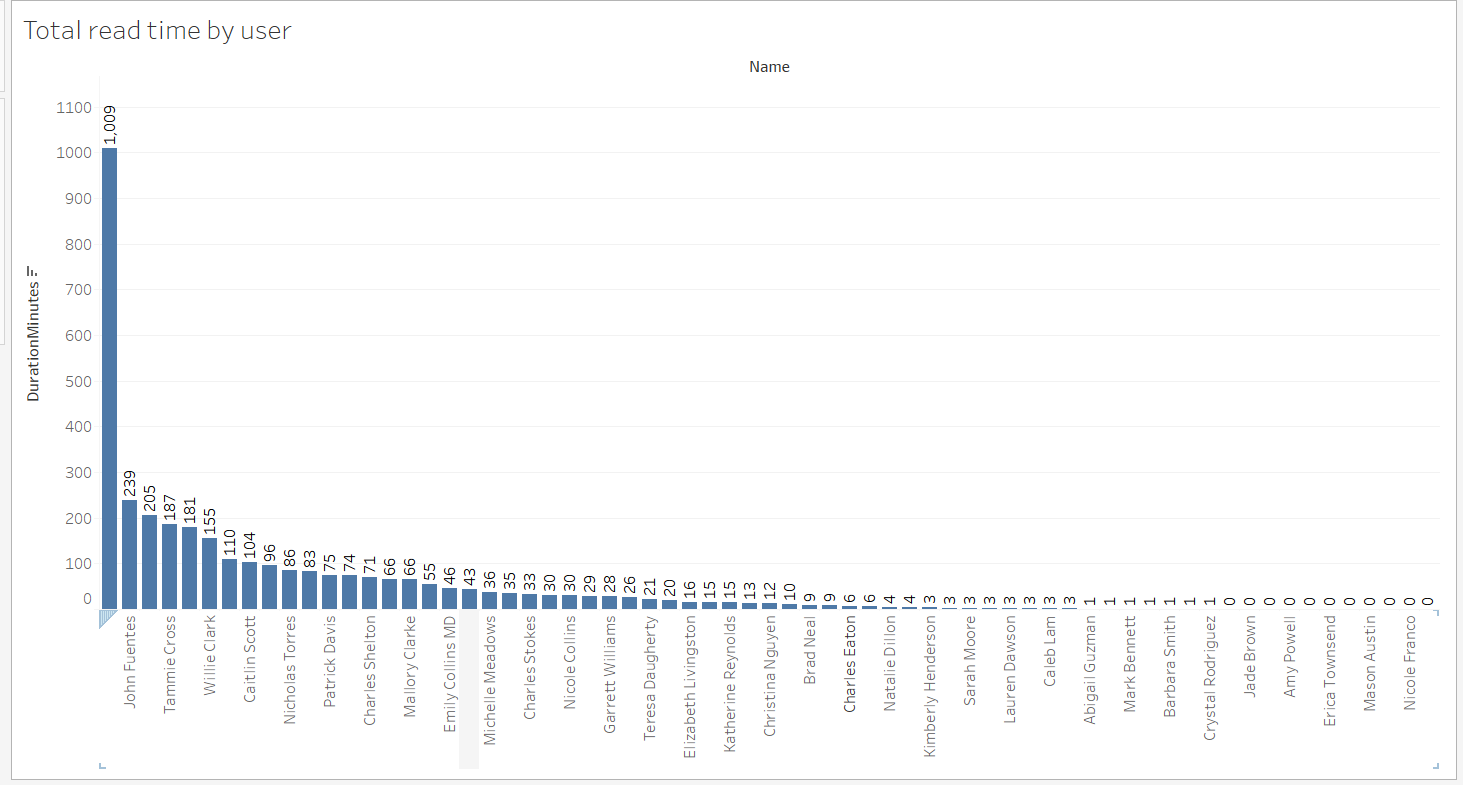
\includegraphics[width=.45\linewidth]{gfx/total_read_time_2_min_scroll}\label{fig:total_read_time_2_min_scroll}} \quad 
	\subfloat[Average read time by user]
	{
		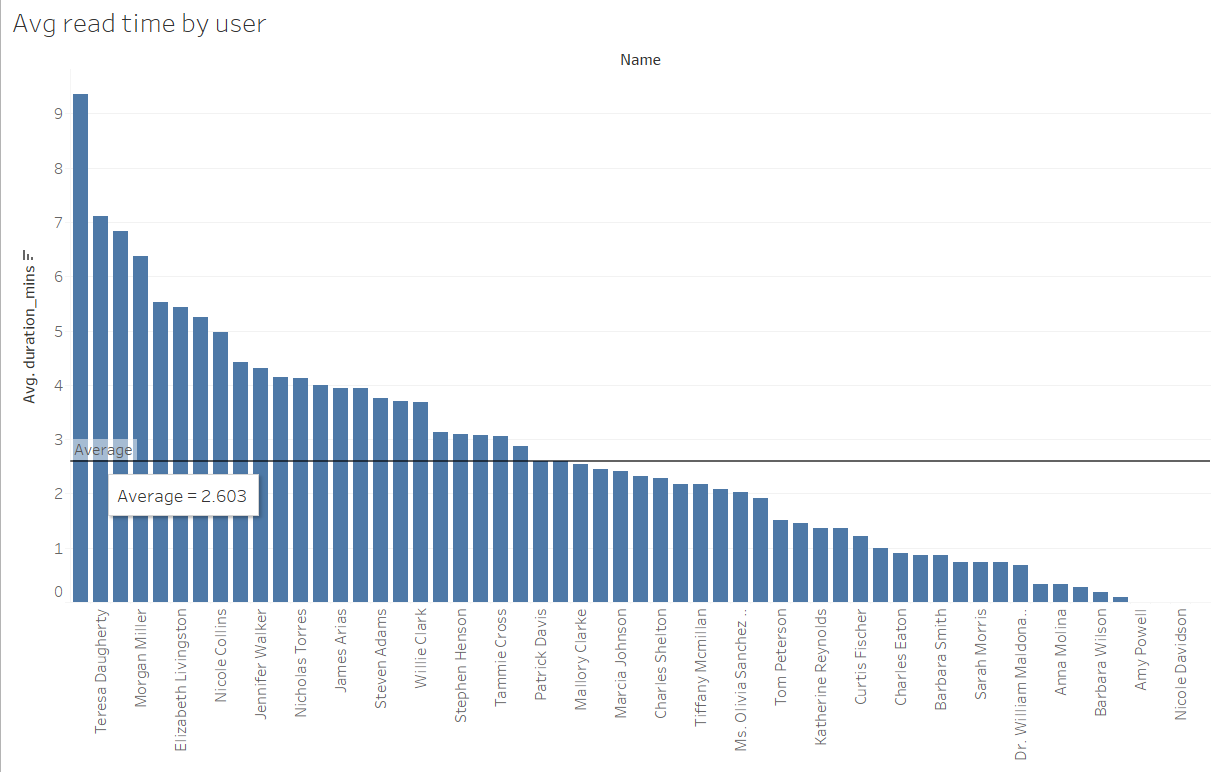
\includegraphics[width=.45\linewidth]{gfx/avg_read_time_2_min_scroll}\label{fig:avg_read_time_2_min_scroll}} \\
	\subfloat[Daily activity timeline]
	{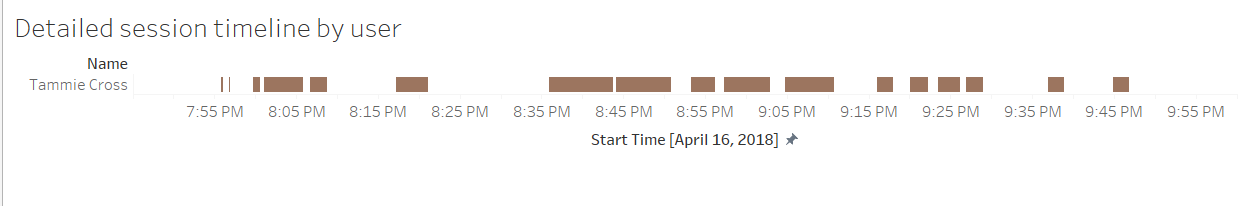
\includegraphics[width=.75\linewidth]{gfx/detailed_session_timeline_by_user_2min_scroll}\label{fig:detailed_session_timeline_by_user_2min_scroll}} \quad
	\caption{Reading session visualizations for session\_timeout of 2 minutes.}\label{fig:visualizations_2nd_iteration}
\end{figure}

By observing figure \ref{fig:total_read_time_2_min_scroll} and comparing it to the results obtained in figure \ref{fig:total_read_time_5min_no_scroll}, we find a clear change in the total reading time by user, the largest amount was 2120 minutes while now the largest is 1009. A similar behavior is observed for the rest of the observations, this tells us that the previous session\_timeout value was too big, therefore computing times longer than what they really were.

For the average reading time by user plot, we observe that the values do not change much from the previous results (figures \ref{fig:avg_read_time_2_min_scroll} vs \ref{fig:avg_read_time_5_min_no_scroll}). The longest average time is now 9 minutes instead of 11. However, now the mean of all the values moved op to 2.6 minutes, which tells us that the value of 2 minutes is smaller than what we need.

Finally, for the detailed activity, a big change is observed, in figure \ref{fig:detailed_session_timeline_by_user_5min_no_scroll}, we observe roughly two smooth reading sessions, which now with a finer session detection broke down into smaller reading sessions (figure \ref{fig:detailed_session_timeline_by_user_2min_scroll}). This means that we correctly detected the user's gap of attentions, therefore a more precise session time was measured.

After the initial findigs, the session tracking calculation was run with different parameters to find the best settings. In table \ref{tb:read_session_timeouts}, the average session durations are compared.

\begin{table}[htb]
	\begin{tabularx}
		{\textwidth}{Xll}\toprule
		\tableheadline{Session\_timeout value} & \tableheadline{Avg. read session (in minutes)} \\ 
		\midrule 
		1 & 1 \\ 
		\hline 
		2 & 1 \\ 
		\hline 
		2.6 & 3 \\ 
		\hline 
		3.2 & 4 \\ 
		\hline 
		4 & 4 \\ 
		\hline 
		5 & 5 \\ 
		\hline 
	\end{tabularx} 
	\caption{Average read sessions duration with different values of session\_timeout}\label{tb:read_session_timeouts}
\end{table}

As we can observe for the average session time, for low values, the average session duration decreases because the sessions are being split into smaller chunks. And for high values, the small sessions are stitched, thus moving the average to a higher value. However, for values between 2 and 4 minutes, we observe that the average stabilizes, therefore we use the value of 4 minutes as the final reading \textbf{session\_timeout}.


By running the reading session computations with the session timeout of 4 minutes, we observe an increase in the total time by around 30\% but still not as much as the baseline (figure \ref{fig:total_read_time_4_min}). The average reading time stabilizes at 4 minutes (figure \ref{fig:avg_read_time_4_min}). And the detailed time line sessions end up in an intermediate outcome between the two previous examples (figure \ref{fig:detailed_session_timeline_by_user_4min}).

\begin{figure}[bth]
	\myfloatalign
	\subfloat[Total read time by user]
	{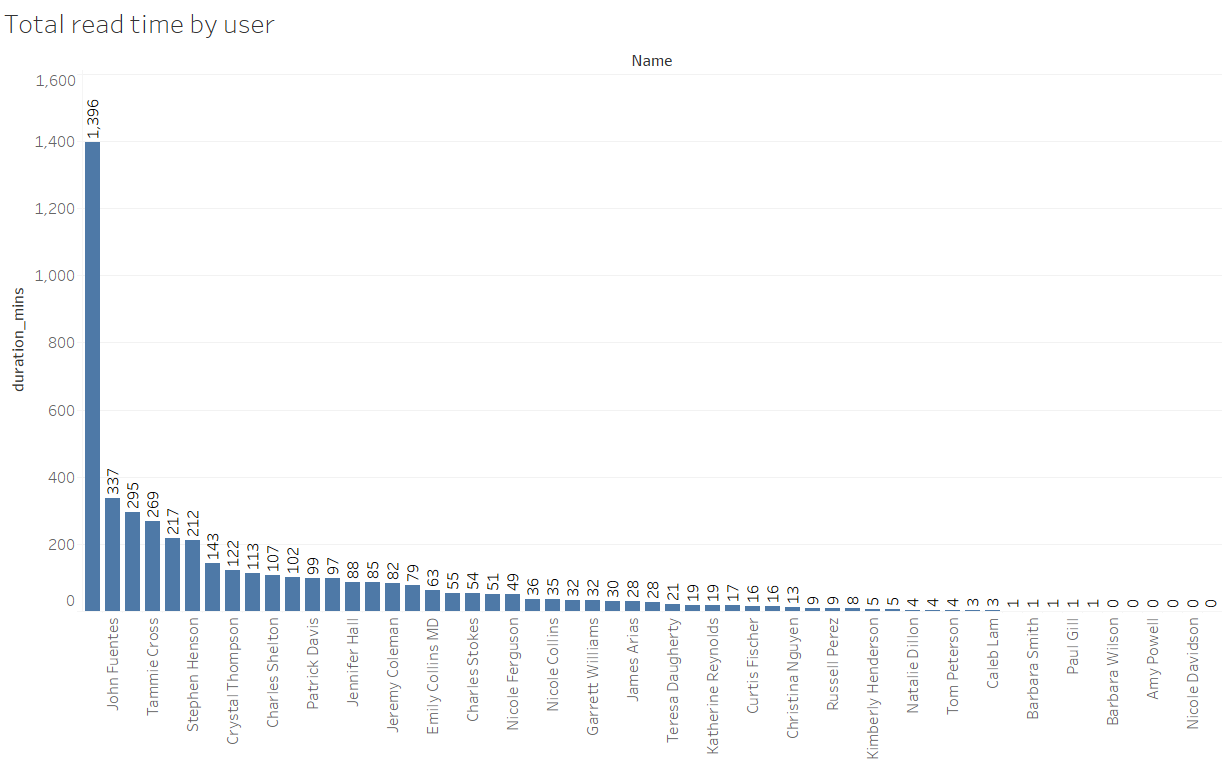
\includegraphics[width=.45\linewidth]{gfx/total_read_time_4_min}\label{fig:total_read_time_4_min}} \quad 
	\subfloat[Average read time by user]
	{
		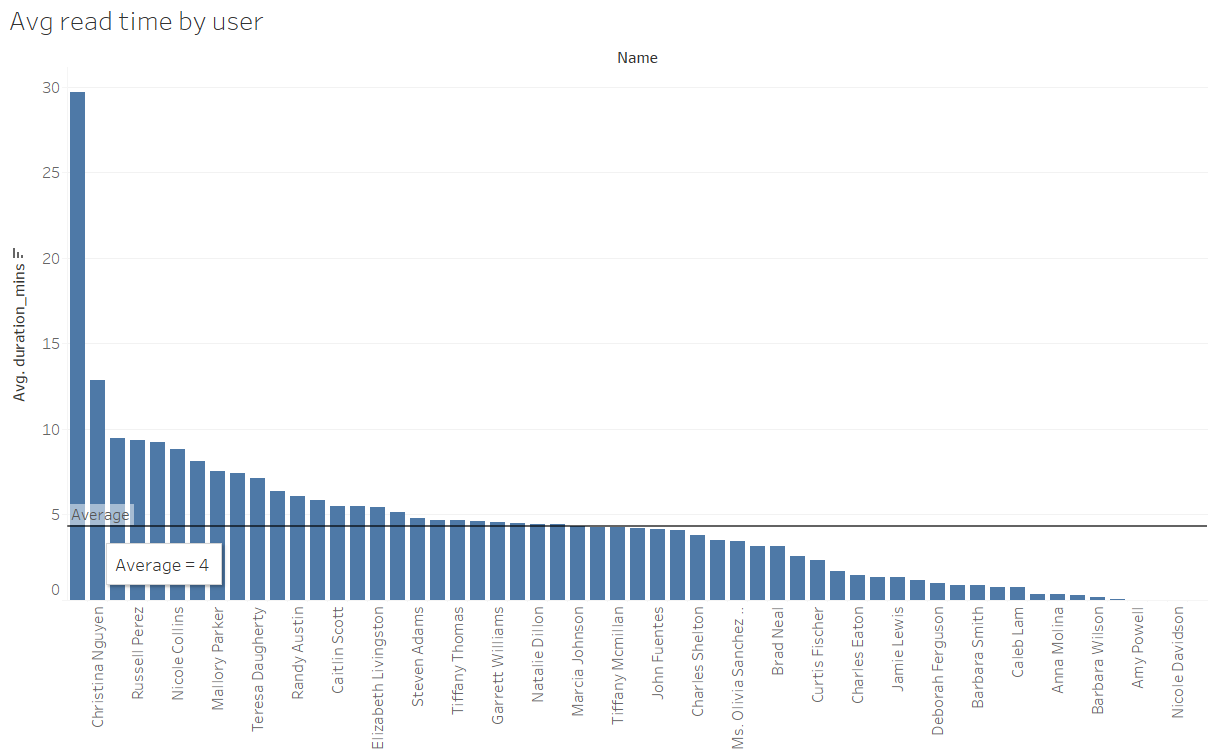
\includegraphics[width=.45\linewidth]{gfx/avg_read_time_4_min}\label{fig:avg_read_time_4_min}} \\
	\subfloat[Daily activity timeline]
	{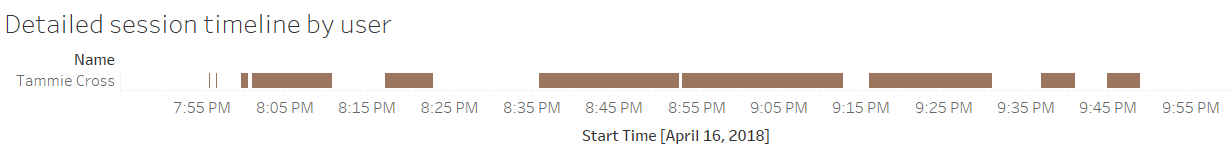
\includegraphics[width=.75\linewidth]{gfx/detailed_session_timeline_by_user_4min}\label{fig:detailed_session_timeline_by_user_4min}} \quad
	\caption{Reading session visualizations for session\_timeout of 4 minutes.}\label{fig:visualizations_last_iteration}
\end{figure}

\section{Exercise session experiments}
For the exercise sessions, the implementation is quite simple, the only event that we track is answering of the exercise (either right or wrong or event asking for a hint). Therefore the only parameter to define is the exercise session\_timeout. For the exercises, we know that they are short and quick activities, which take only a couple of second to provide an answer. Therefore the timeout must be much smaller than for reading.

Again, a series of experiments were run with different settings to detect the optimal timeout value. In table \ref{tb:exercise_session_timeouts} we can observe the average exercise session length computed for different parameters of the session\_timeout.


%Table of tests
\begin{table}[htb]
	\begin{tabularx}
		{\textwidth}{Xll}\toprule
		\tableheadline{Session\_timeout value} & \tableheadline{Avg. session (in minutes)} \\ 
		\midrule 
		1 & 2.7 \\ 
		\hline 
		2 & 3.7 \\ 
		\hline 
		2.5 & 4 \\ 
		\hline 
		3 & 4.2 \\ 
		\hline 
		4 & 4.7 \\ 
		\hline 
		5 & 5.22 \\ 
		\hline 
	\end{tabularx} 
	\caption{Comparative of the average session duration using different session\_timeout values for exercises}\label{tb:exercise_session_timeouts}
\end{table}

Based on results, it is difficult to find a clear winning value, however, fluctuations decrease around a value of 4 minutes. Of course, if we keep increasing the value, we would find longer sessions, but since we want to be as strict as possible, a value of 4 is chosen as the optimal.


\section{Dashboard}
TO BE DEFINED